
\begin{figure}[h]
    \centering
    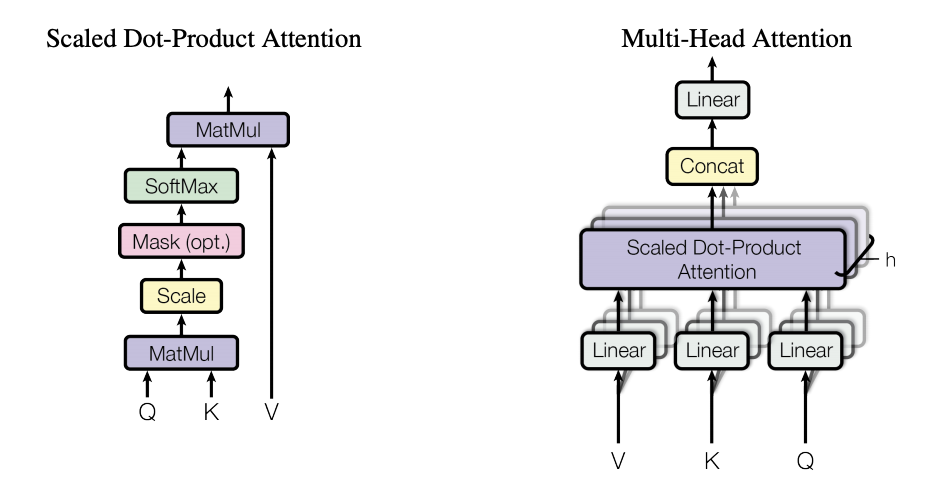
\includegraphics[width=.9\linewidth]{figs/selfattention.png}
    \caption{Flowchart of the main component of the transformer, self-attention.}
    \label{fig:selfattention}
\end{figure}


\section{Vision Transformer}\label{sects:Transformer}

In this section, we are going to expose the inner workings of the Transformer architecture. Recall that it was introduced for NLP tasks. Often, sentences have words of which the meaning is dependent on their context. This is the problem that the transformer tries to address. Firstly, words are encoded into embeddings which capture their isolated semantic. Next, words are mixed with each other using self-attention. Self-attention, is an attention-mechanism where elements in a sequence are combined together based on their similarity. Intuitively, a word attends to (meaning "pays attention to") other similar words in the sentence. When a word $u$ attends to a word $v$ collects and incorporates the embedding of $v$ into its own. Practically, $u$ incorporates the meaning of $v$ into itself. After several iterations of this mechanism a word obtains an embedding that it is not only representative of its own semantics, but also, it is representative of its surrounding. 

An example may help to understand both the problem and the solution. Consider the phrase "bank of a river". The word "bank" alone has a semantic that is very different from the semantic that has in this phrase. During the previous steps of the transformer. The embedding of "bank" would get mixed with the embedding of "river" in such a way that, "bank" becomes representative of the contextual meaning of the word. Another way of seeing the same approach is the following: Some \textit{complex meanings} can be only obtained by combining other \textit{simple meanings} together. Self-attention is a mechanism for combining meanings.

Now, let us introduce the architecture by starting from the input. The Transformer takes as input $n$ embeddings of size $d$. In our case, embeddings will be patches of an image, as shown by Fig.~\ref{img:patches}. Let us call $X = [x_1, \dots, x_n] \in \mathbb{R}^{n\times d}$. Now that we have our patches, we can feed them to the first Transformer Encoder layer. Let us introduce three parameter matrices $W_Q, W_K, W_V \in \mathbb{R}^{n\times d}$. We proceed to compute the so-called queries, keys, and value vectors (shown as inputs in Fig.~\ref{fig:selfattention}):
\[Q = X^T\cdot W_Q, K = X^T\cdot W_K, V = X^T\cdot W_V\]
Once we have computed these matrices representing three different linear transformations of the input, we proceed by applying the so-called self-attention (shown in \ref{fig:selfattention}). But firstly, let us introduce the softmax non-linearity. The softmax function takes as input a vector $v \in \mathcal{R}^{1\times k}$ and outputs a vector $v' \in \mathcal{R}^{1\times k}$ such that $\sum_i v'_i = 1$ and $v_i \leq v_j \implies v'_i \leq v'_j \forall i,j$:
\[softmax(v)_i = \frac{e^v_i}{\sum_j{e^v_j}}, v'=[softmax(v)_1,\dots,softmax(v)_k]\]
Finally, we can compute the self-attention (depicted as Scaled Dot-Product Attention in Fig.~\ref{fig:selfattention}):
\[Z = softmax(\frac{Q\cdot K^T}{\sqrt{d}})\cdot V\]
This represents the heart of the Transformer architecture. By $Q \cdot K^T$, we are computing the dot product between each row-vector in $Q$ and each row-vector in $K$. This returns a similarity matrix scoring each query against each key. Afterward, we turn these scores (by applying the softmax function row-wise) into probability distributions. By now, we have a probability distribution for each patch in our image. Each probability distribution tells us how similar is a patch wrt. the others. The last matrix multiplication is going to use these distributions to sum all the patches weighted by the probability score. Ultimately, self-attention is a way to reroute information between vectors based on their similarity.
The last component of the encoder layer applies a standard feed-forward network and a skip connection with the original input. Now, multiple encoders can be stacked together to achieves, usually, higher results.

You may have noticed that the Transformer Encoder has no way of knowing if a patch comes from the center of the image or comes from the left corner of the image. To mitigate this issue, we introduce positional embeddings. These are simply parameter vectors $[e_1, \dots, e_n]\in\mathcal{R}^{d\times n}$. These vectors are meant to represent positions and are summed altogether with our input. We can redefine the Transformer Encoder input as follows:
\[X = [x_1+e_1,\dots,x_n+e_n]\]

Another important component is the Transformer Decoder. However, the final architecture of this project will not be used. Thus, we are not discussing this component. Nonetheless, additional material about the transformer can be found \url{http://jalammar.github.io/illustrated-transformer/}.

With these considerations, our overview of the Transformer architecture is complete.
\begin{figure}
    \begin{subfigure}{.5\textwidth}
        \centering
        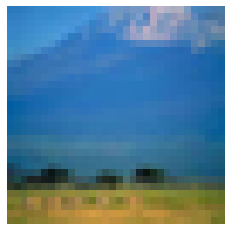
\includegraphics[width=.9\linewidth]{figs/fullimage.png}
        \subcaption{full image}
    \end{subfigure}
    \begin{subfigure}{.5\textwidth}
        \centering
        
\includegraphics[width=.9\linewidth]{figs/patchedimage.png}
        \subcaption{image divided in $12\times12=n$ patches}
    \end{subfigure}
    \caption{both figures are taken from the Keras vision transformer tutorial available at \url{https://keras.io/examples/vision/image_classification_with_vision_transformer/}}
    \label{img:patches}
\end{figure}


